\subsection{Progettazione architetturale}
\textit{\textbf{Periodo}: dal 2021-01-18 al 2021-03-08}

L'inizio di questa fase coincide con la data della Revisione dei Requisiti e si conclude con la scadenza della Revisione di Progettazione.

\subsubsection{Attività}

\begin{itemize}
\item \textbf{Incremento e verifica documenti}: vengono realizzati gli incrementi necessari ai documenti. I documenti in questione sono:
\begin{itemize}
\item \NdP{};
\item \AdR{};
\item \PdQ{};
\item \PdP{};
\item Glossario.
\end{itemize}
\item \textbf{Technology Baseline\ped{G}}: viene realizzato un \textit{Proof of Concept}\ped{G} per testare le tecnologie coinvolte e per provare che le funzionalità base del prodotto possano effettivamente essere implementate, soddisfacendo i requisiti collegati. Esso verrà condiviso con il proponente, per verificare che sia soddisfacente, e con il \CR{}.\\ Come precedentemente notato, nella sezione \S{3.2}, per la realizzazione del \textit{Proof of Concept}\ped{G} sono stati individuati quattro incrementi, che suddividono lo sviluppo e la realizzazione della documentazione in aree di interesse distinte. Per ogni incremento vengono riportati i requisiti che ci impegniamo a soddisfare nel \textit{Proof of Concept}\ped{G} (non comprendendo i requisiti figlio):
\begin{itemize}
\item \textbf{Incremento 1}: R1F1;
\item \textbf{Incremento 2}: R1F7.1, R1F9.1;
\item \textbf{Incremento 3}: R1F4;
\item \textbf{Incremento 4}: R1F11.
\end{itemize}
Questa lista di requisiti non esclude il fatto che possano essere soddisfatti altri requisiti aggiuntivi.
\item \textbf{Consolidamento}: viene realizzata la presentazione da esporre in sede di Revisione di Progettazione e si approfondiscono aspetti lacunari riguardo il progetto.
\end{itemize}

\subsubsection{Periodi}

\begin{itemize}
\item \textbf{Periodo 1}: \textit{dal 2021-01-18 al 2021-01-31}. \\
Viene svolto un approfondimento personale da ogni membro del gruppo riguardo le tecnologie da utilizzare per lo sviluppo del prodotto. Inoltre verranno incrementati i documenti realizzati nella fase di analisi.
\item \textbf{Periodo 2}: \textit{dal 2021-01-31 al 2021-03-01}. \\
Viene realizzata la Technology Baseline\ped{G}, compresa di un'analisi iniziale degli incrementi e delle tecnologie, la realizzazione degli incrementi e una verifica finale di integrazione. Di seguito vengono riportati i periodi individuati per i singoli incrementi:
\begin{itemize}
\item \textbf{Incremento 1}: \textit{dal 2021-02-04 al 2021-02-09};
\item \textbf{Incremento 2}: \textit{dal 2021-02-09 al 2021-02-14};
\item \textbf{Incremento 3}: \textit{dal 2021-02-14 al 2021-02-19};
\item \textbf{Incremento 4}: \textit{dal 2021-01-19 al 2021-02-24}.
\end{itemize}
Il periodo si conclude con la consegna del materiale per la Revisione di Progettazione;
\item \textbf{Periodo 3}: \textit{dal 2021-03-01 al 2021-03-08}. \\
Viene svolta l'attività di consolidamento. Il periodo si conclude con la Revisione di Progettazione;
\end{itemize}

\subsubsection{Diagramma di Gantt}

\begin{figure}[H]
\centering

\centerline{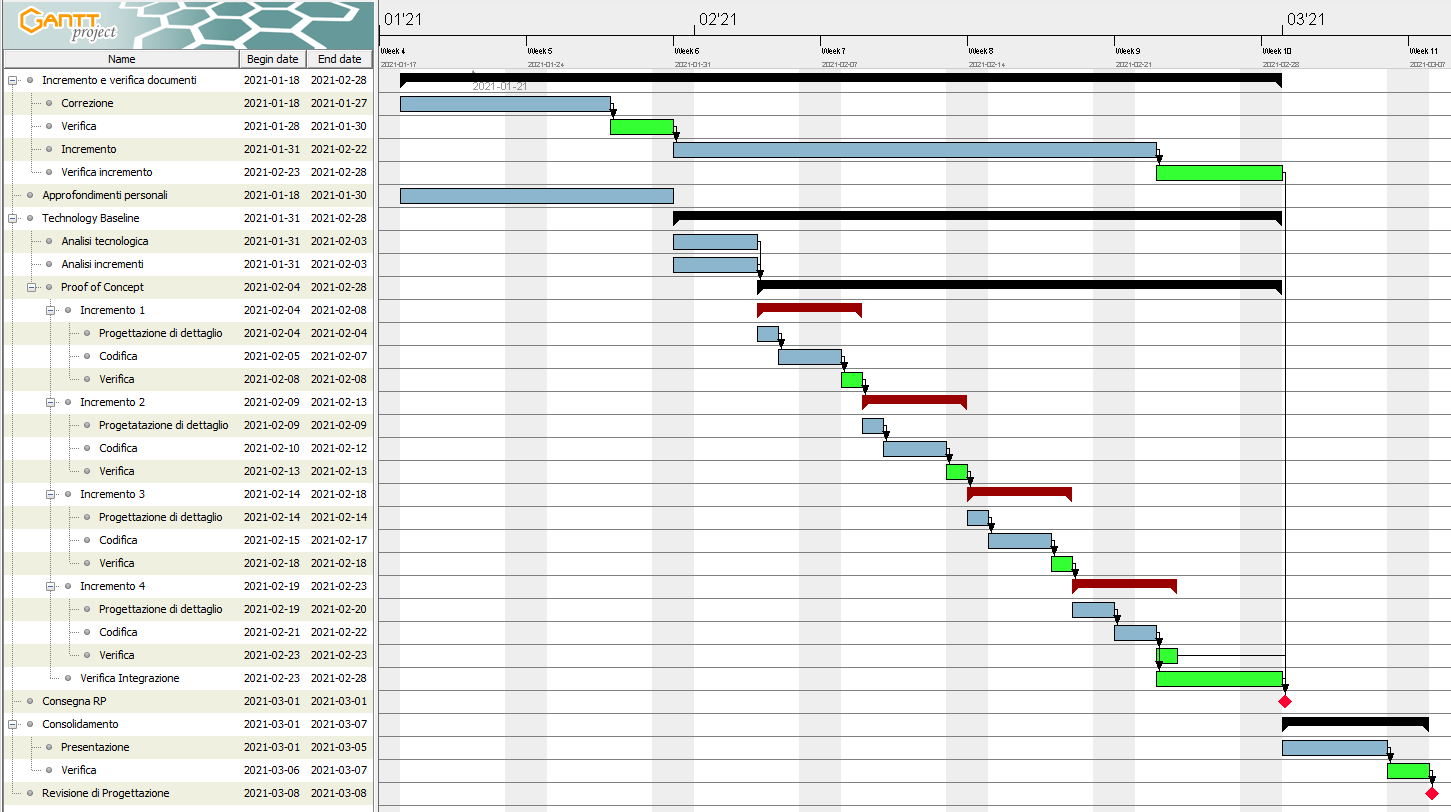
\includegraphics[scale=0.5]{res/Pianificazione/Gantt/progettazione}}
\caption{Diagramma di Gantt per il periodo di progettazione architetturale}
\end{figure}

Per migliorare la visualizzazione del diagramma, la pianificazione dei singoli incrementi viene rappresentata dal successivo diagramma, che ha una durata di 5 giorni.\\

\begin{figure}[H]
\centering

\centerline{\includegraphics[scale=1]{res/Pianificazione/Gantt/incrementoProgettazione}}
\caption{Diagramma di Gantt per i singoli incrementi nel periodo di progettazione architetturale}
\end{figure}